\documentclass[12pt, a4paper]{report}
%------------------------------------------------------------------------------
%------------------------------------------------------------------------------
% PACKAGES
%------------------------------------------------------------------------------

\usepackage[utf8]{inputenc}
\usepackage{amsmath}
\usepackage{amsfonts}
\usepackage{amssymb}
\usepackage{graphicx}
\usepackage{wrapfig}
\usepackage{float}
\usepackage{caption}
\usepackage[italian]{babel}
\usepackage[hmargin={2.3cm,2.3cm},vmargin={3cm,3cm}]{geometry}
\usepackage[]{hyperref}
%\usepackage{fontspec}

%------------------------------------------------------------------------------
% TITLE PAGE
%------------------------------------------------------------------------------

\author{
\LARGE
Valerio Casalino \\ 
\LARGE
233808 
}

\title{ 
\Huge
\textbf{Relazione di Elaborazione dei Segnali} \\ 
\LARGE
Politecnico di Torino AA 2018-2019 \\
\vspace*{2cm} 

\includegraphics[width=.5\textwidth]{images/logo.png}
}

\date{}

%------------------------------------------------------------------------------
% DOCUMENT
%------------------------------------------------------------------------------

\begin{document}

\maketitle

\cleardoublepage
\tableofcontents

\chapter{Introduzione}
%------------------------------------------------------------------------------
\section{Obiettivi e traguardi}
L'obiettivo delle esercitazioni è quello di mettere in pratica, osservare e 
verificare il livello di apprendimento della materia appoggiandoci 
sull'ambiente MATLAB 
\href{https://it.mathworks.com/products/matlab.html}{[Website link]}.

%-------------------------------------------------------------------------------
\section{Materiale e documentazione disponibile}
Abbiamo a disposizione per lo svolgimento delle esercitazioni, oltre che alle 
conoscenze pregresse, anche il seguente materiale:
\begin{itemize}
    \item Documentazione interna di MATLAB, attraverso i comandi \textit{doc} e 
    \textit{help}.
    \item La sezione dedicata su StackOverflow: 
    \url{https://stackoverflow.com/questions/tagged/matlab}.
    \item La community di MATLAB: 
    \url{https://it.mathworks.com/matlabcentral/?s_tid=gn_mlc}.
\end{itemize}

%-------------------------------------------------------------------------------
\section{Note}
La relazione, come i codici sorgente delle esercitazioni, sono disponibili su 
GitHub, all'indirizzo \url{http://bit.ly/vcasalino-github-tes}. 

\chapter{LAB1: Convoluzione, mutua correlazione e stima del ritardo}
\section{Convoluzione Lineare}

\begin{quote}
	\emph{In matematica, in particolare nell'analisi funzionale, la convoluzione è un'operazione tra due funzioni di una variabile che consiste nell'integrare il prodotto tra la prima e la seconda traslata di un certo valore. }
\end{quote}
\hspace*{\fill} \href{https://it.wikipedia.org/wiki/Convoluzione}{-Wikipedia}. \\

L'operazione di convoluzione tra funzioni continue è definita in tale modo:
\begin{equation}
	f \circledast g = \int^{\infty}_{- \infty} f(\tau)g(t-\tau)d\tau = \int^{\infty}_{- \infty} f(t - \tau)g(\tau)d\tau
\end{equation}

La convoluzione discreta, invece, è definita come:
\begin{equation}
	\sum^{\infty}_{m= - \infty} f[m]g[n-m] = \sum^{\infty}_{m= - \infty} f[n-m]g[m] 
\end{equation}


\chapter{LAB2: Discrete Fourier Transform}
%-------------------------------------------------------------------------------

\section{Esercizio 1: Convoluzione e sistemi LTI}
La convoluzione tra due segnali è equivalente al loro prodotto nel dominio 
della frequenza. Possiamo riscrivere la funzione di convoluzione dell'esercizio
precedente sfruttando questa relazione matematica:

\begin{equation}
	z(n) = x(n) \circledast y(n) \rightarrow 
	z(n) = F^{-1}(F[x(n)](f) \cdot F[y(n)](f))	
\end{equation}

%-------------------------------------------------------------------------------

\section{Implementazione DFT}
In MATLAB è possibile implementare le DFT e le IDFT come segue:

		
\begin{equation}
	x_{out}[k] = \begin{cases} 
	
	\frac{1}{N} \sum^{N-1}_{n=0} x_{in}[n] 
	e^{j 2 \pi k n / N } & k=0,...,N-1 \\ 
	
	\sum^{N-1}_{n=0} x_{in}[n] 
	e^{- j 2 \pi k n / N } & k=0,...,N-1 
	
	\end{cases}
\end{equation}

dove N è la lunghezza del segnale $x_{in}[n]$.

%-------------------------------------------------------------------------------

\begin{minipage}[t]{.45\textwidth}
	\begin{figure}[H]
	\centering
	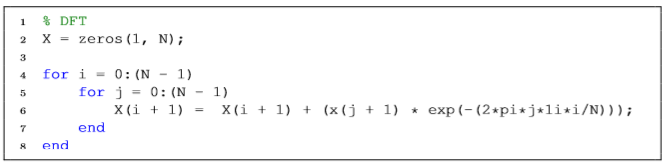
\includegraphics[width=\textwidth]{./images/cap3/DFT.png}
	\caption{Implementazione DFT.}
\end{figure}
\end{minipage}
\hfill
\begin{minipage}[t]{.45\textwidth}
	\begin{figure}[H]
	\centering
	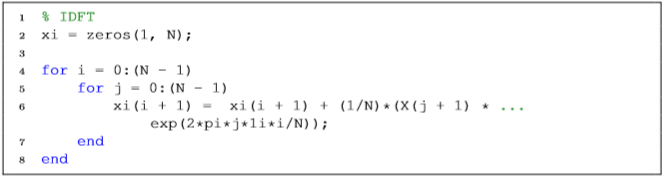
\includegraphics[width=\textwidth]{./images/cap3/IDFT.png}
	\caption{Implementazione IDFT.}
\end{figure}	
\end{minipage}

\pagebreak

Le funzioni implementate in questo modo risultano essere equivalenti alle 
funzioni di libreria \textit{fft()} e \textit{ifft()} implementate in MATLAB, 
come si vede in figura \ref{fig:output_L2E2}.

\begin{figure}[H]
\centering
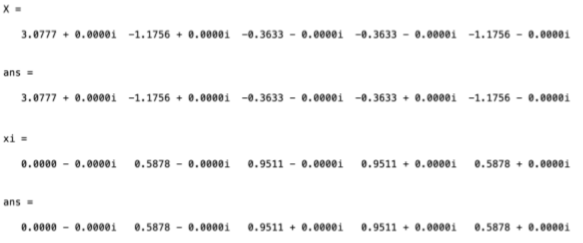
\includegraphics[width=.75\textwidth]{./images/cap3/output_L2E2.png}
\caption{Output MATLAB Esercizio 2.}
\label{fig:output_L2E2}
\end{figure}

\section{DFT di segnali analogici}
A partire da un segnale nel tempo $x(t)$ è possibile simularne una versione 
campionata nell’intervallo frequenza di campionamento:

\begin{equation}
	f_c = \frac{1}{T_0}
\end{equation}

nel seguente modo:

\begin{equation}
	x[n] = x(nT_c)
\end{equation}

dove $N=T_0 f_c$ è il numero di campioni. Si considerano, dunque, i seguenti 
segnali:

\begin{itemize}
	\item $x(t) = sinc^2 (t)$
	\item $x(t) = e^{-4|t|}$
	\item $x(t) = cos(2 \pi t)$
\end{itemize}

%-------------------------------------------------------------------------------

Dato un intervallo di durata $T_0 = 4$ secondi, si procede a campionare i 
segnali con due diverse frequenze di campionamento $fc = 5 Hz$ e $fc = 20$ 
Hz e a calcolarne la DFT.

\begin{minipage}[t]{.6\textwidth}
	\begin{figure}[H]
		\centering
		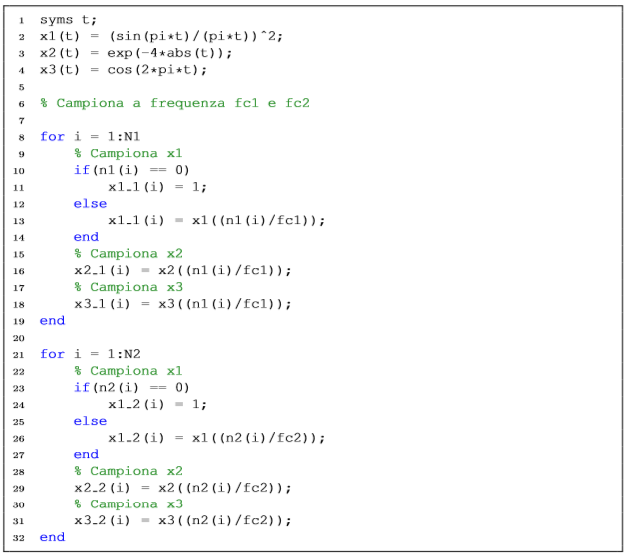
\includegraphics[width=\textwidth]{./images/cap3/campionamento_iterativo.png}
	\end{figure}
\end{minipage}
\hfill
\begin{minipage}[t]{.3\textwidth}
	\vspace*{1cm}
	Una volta generate le funzioni in MATLAB mediante l’utilizzo di una variabile 
	simbolica t è possibile procedere al campionamento iterativo dei segnali, dopo 
	avere preventivamente allocato dei vettori di dimensione opportuna negli 
	intervalli relativi a $N_1$ e $N^2$:
\end{minipage}

\bigskip

Fatto ciò è possibile rappresentare su un grafico il modulo delle trasformate 
di Fourier sei segnali campionati.

\begin{figure}[H]
	\centering
	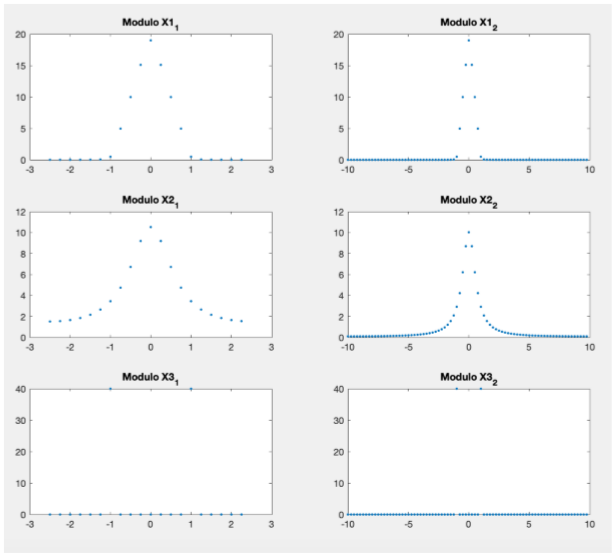
\includegraphics[width=.7\textwidth]{./images/cap3/segnali_campionati.png}
\end{figure}

E possibile notare come la maggior frequenza di campionamento associata alla 
parte destra del grafico implichi una maggior precisione nel disegno della 
trasformata di Fourier dei segnali presi in considerazione.

\chapter{LAB3: Periodogrammi}
%-------------------------------------------------------------------------------
\section{Introduzione}
Dati N campioni di un processo casuale stazionario $x(n)$, la stima spettrale è 
l’operazione che consente di stimare la sua densità spettrale di potenza 
$S_X(f)$. La disponibilità di un numero finito di campioni del segnale è, però, 
un fattore che va tenuto in considerazione, dato che influisce sulla risoluzione 
e affidabilità della stima. L’operazione più semplice di stima spettrale è il 
periodogramma, basato sulla DFT.
\par
Selezioniamo, quindi, un file audio tra quelli proposti in sede di laboratorio 
tutti campionati a $f_s = 44100 Hz$. Una volta importati in MATLAB usando la 
funzione audioread, selezionarne una porzione di durata 1 e 5 secondi 
(corrispondente a $N = 44100$ e 5N campioni), chiamata $x(n)$: 

\begin{figure}[H]
	\centering
	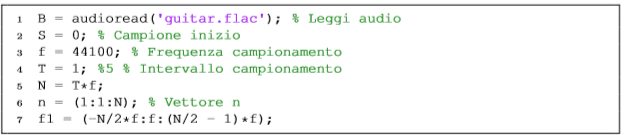
\includegraphics[width=.8\textwidth]{./images/cap4/acquisizione.png}
\end{figure}

\section{Periodogramma Semplice}
Una volta acquisito correttamente $x(n)$ è possibile valutarne il periodogramma 
semplice mediante la definizione e la libreria di MATLAB \textit{ftt()}:

\begin{minipage}[t]{.25\textwidth}
	\vspace*{.75cm}
	\begin{equation*}
	P_X (k) = \frac{|X(k)|^2}{N}
	\end{equation*}
\end{minipage}
\hfill
\begin{minipage}[t]{.7\textwidth}
	\begin{figure}[H]
		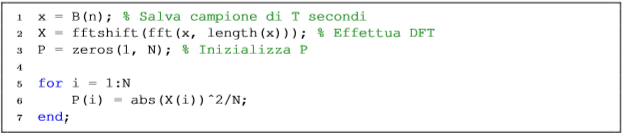
\includegraphics[width=\textwidth]{./images/cap4/ifft.png}
	\end{figure}
\end{minipage}

\bigskip

Una volta calcolati i periodogrammi per uno e cinque secondi di registrazione, 
è possibile disegnarli mediante il comando \textit{plot()} di MATLAB e 
valutarne le differenze:

\begin{minipage}[t]{.45\textwidth}
	\begin{figure}[H]
		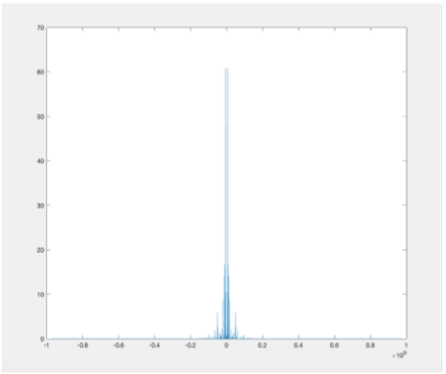
\includegraphics[width=\textwidth]{./images/cap4/per1s.png}
		\caption{Periodogramma per 1 secondo di registrazione.}
	\end{figure}
\end{minipage}
\hfill
\begin{minipage}[t]{.45\textwidth}
	\begin{figure}[H]
		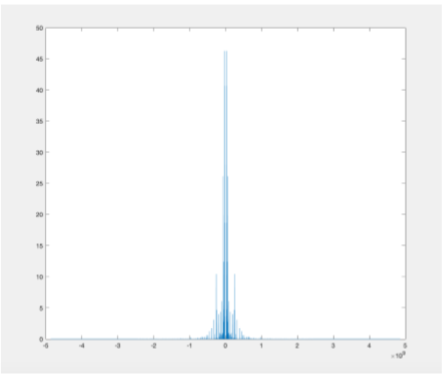
\includegraphics[width=\textwidth]{./images/cap4/per5s.png}
		\caption{Periodogramma per 5 secondi di registrazione.}
	\end{figure}
\end{minipage}

Si può affermare che il periodogramma valutato su un intervallo di cinque 
secondi risulta più fitto e mostra un maggior numero di contenuto 
in frequenza.

%-------------------------------------------------------------------------------

\section{Periodogramma di Barlett}
Come osservato nel punto precedente, il periodogramma semplice ha elevata 
risoluzione in frequenza ma è “rumoroso”. Una tecnica per ridurre il rumore è 
eseguire il cosiddetto periodogramma di Bartlett, ottenuto dividendo la 
sequenza x(n) in M intervalli disgiunti di $N/M$ campioni 
ciascuno, calcolando il periodogramma di ciascuna sottosequenza e 
mediando il risultato.
\begin{minipage}[t]{.35\textwidth}
	\begin{figure}[H]
		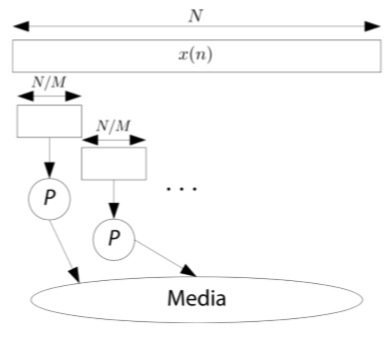
\includegraphics[width=\textwidth]{./images/cap4/barlett.png}
	\end{figure}
\end{minipage}
\hfill
\begin{minipage}[t]{.55\textwidth}
	\vspace*{2cm}
	\begin{equation*}
		P_X(k) = \frac{1}{M} \sum^{M-1}_{i=0} \frac{|X^{(i)}(k)|^2}{N/M}
	\end{equation*}
\end{minipage}

\bigskip

dove $X_{(i)}(k)$ è la DFT dell'i-esimo intervallo $x(n)$. Una volta 
acquisito correttamente x(n) è possibile valutarne il periodogramma di 
Bartlett mediante la definizione per valori $M = 10, 50, 100$.

\begin{figure}[H]
	\centering
	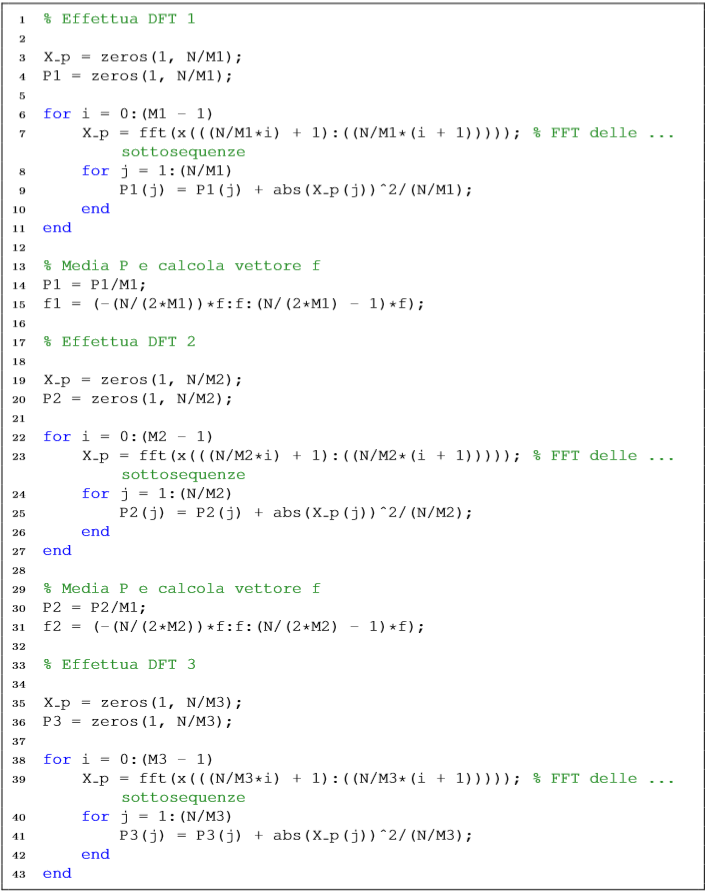
\includegraphics[width=.8\textwidth]{./images/cap4/mat_barlett.png}
\end{figure}

Una volta calcolati i periodogrammi per uno e cinque secondi di registrazione, 
è possibile disegnarli mediante il comando \textit{plot()} di MATLAB e 
valutarne le differenze:

\begin{minipage}[t]{.45\textwidth}
	\begin{figure}[H]
		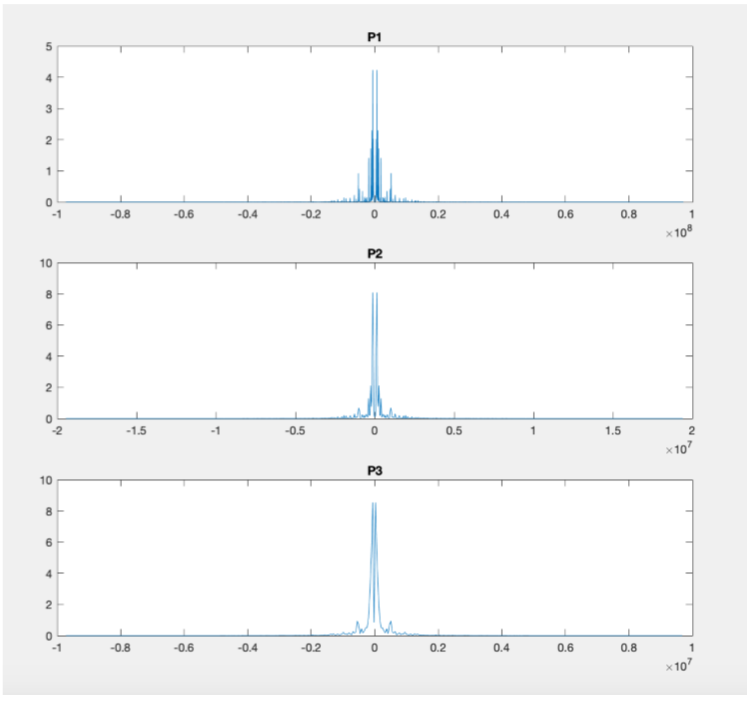
\includegraphics[width=\textwidth]{./images/cap4/barlett1s.png}
		\caption{Periodogramma di Barlett per 1 secondo di registrazione.}
	\end{figure}
\end{minipage}
\hfill
\begin{minipage}[t]{.45\textwidth}
	\begin{figure}[H]
		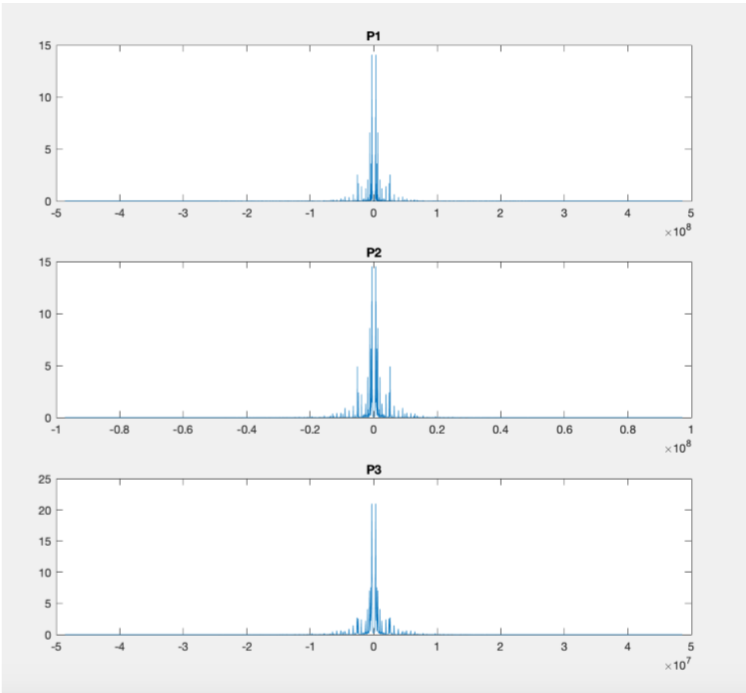
\includegraphics[width=\textwidth]{./images/cap4/barlett5s.png}
		\caption{Periodogramma di Barlett per 5 secondi di registrazione.}
	\end{figure}
\end{minipage}

%-------------------------------------------------------------------------------

\section{Periodogramma di Welch}
Come visto al punto precedente, il periodogramma di Bartlett consente di ridurre 
il “rumore” sulla stima di densità spettrale di potenza, riducendone al contempo 
la risoluzione. Una tecnica più avanzata è il periodogramma di Welch. Rispetto al 
periodogramma di Bartlett, introduce le seguenti modifiche:

\begin{itemize}
	\item Le sotto-sequenze su cui si calcola il periodogramma non sonodisgiunte 
	ma sono sovrapposte del 50\%.

	\begin{figure}[H]
		\centering
		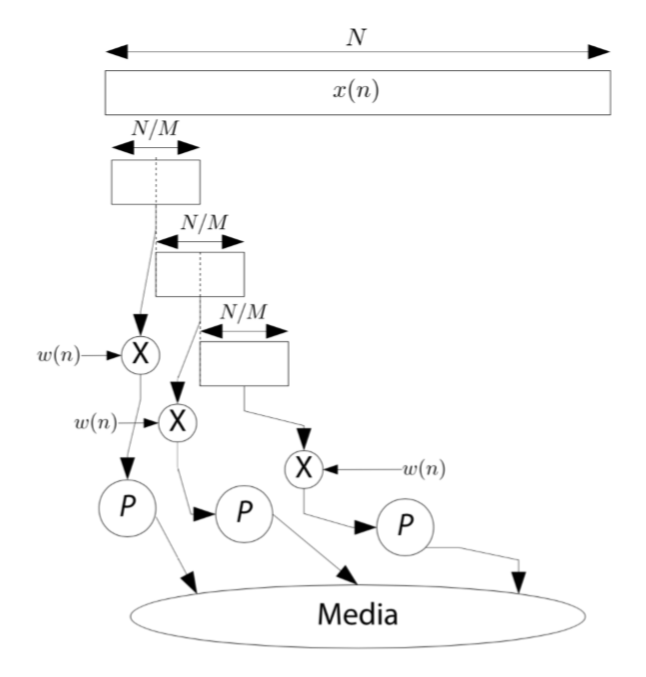
\includegraphics[width=.5\textwidth]{./images/cap4/welch_schema.png}
	\end{figure}

	\item  Prima di eseguire la DFT, ogni sotto-sequenza viene moltiplicata per 
	una funzione $w(n)$ chiamata finestra di Hamming:
	
	\begin{equation*}
		w(n) = \alpha - \beta cos(\frac{2 \pi n}{N/M -1})
	\end{equation*}	
\end{itemize}

La funzione è presente nella libreria di MATLAB sotto il nome di \textit{hamming()}.
Una volta acquisito correttamente x(n) è possibile valutarne il periodogramma di 
Welch mediante la definizione per valori $M = 10, 50, 100$ come fatto per il 
periodogramma di Bartlet.

\begin{figure}[H]
	\centering
	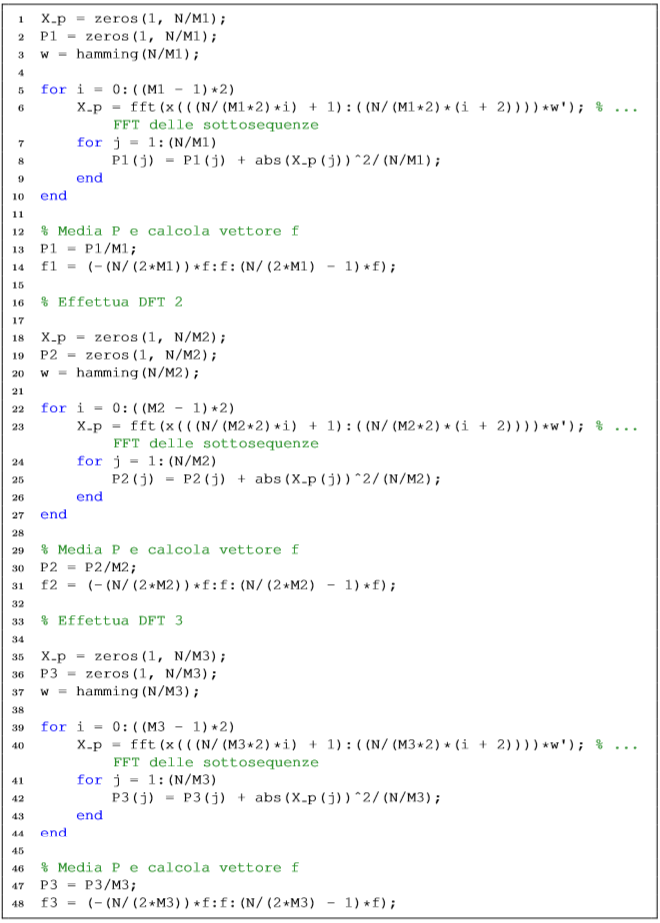
\includegraphics[width=0.7\textwidth]{images/cap4/matlab_welch}
\end{figure}

Eseguendo il periodogramma di Welch della sequenza x(n) usando gli stessi parametri 
usati per il periodogramma di Bartlett `e possibile mettere a confronto i risultati 
ottenuti.

\begin{figure}[H]
	\centering
	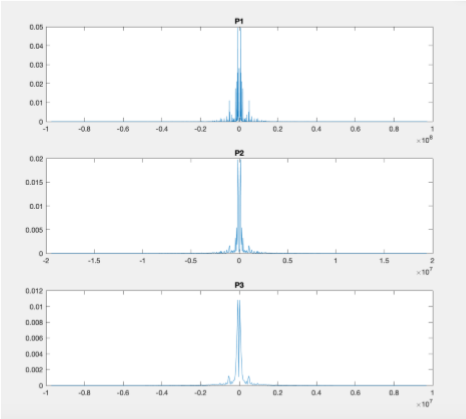
\includegraphics[width=0.7\textwidth]{images/cap4/plot_welch}
\end{figure}


Si nota una riduzione del disturbo nella variazione del periodogramma semplice, 
senza una eccessiva perdita dell’informazione in frequenza.



\end{document}